\chapter{Introduction}
\label{cha:introduction}

% \section{Background}
% Generative models, such as Variational Autoencoders (VAEs) and Generative Adversarial Networks (GANs), aim to learn the underlying distribution of data to create new, synthetic samples. Diffusion models have recently emerged as a powerful class of generative models that produce high-quality data by reversing a progressive noise process. 

% State-of-the-art diffusion models can sometimes generate low-quality samples with artifacts. This can for instance lead to diagnosis errors in medical imaging \parencite{xia_hallucinations_2025}, or in our case, weird\footnote{In this thesis, we define \textit{weird} with regards to human perception and assume that humans are good at deciding if an image belongs to the data distribution} looking natural images \parencite{jazbec_generative_2025}. To identify these failures without manual inspection, Bayesian machine learning principles can be adapted to formulate \textit{generative uncertainty}. It allows to flag poor generations by measuring the variability of the posterior predictive distribution (uncertainty in the model's output). 

% \section{In}

\section{Introduction}

\paragraph{Generative Models}
Generative models, such as Variational Autoencoders (VAEs) and Generative Adversarial Networks (GANs), aim to learn an underlying distribution of data to create new, synthetic samples. Diffusion models have recently emerged as a powerful class of generative models that produce high-quality data by reversing a progressive noise process (\autoref{sec:bg_diffusion}).

\paragraph{The Problem}

State of the art diffusion models can sometimes generate low-quality samples with severe artifacts. In this thesis we look at models generating natural images \parencite{jazbec_generative_2025} where we are mainly concerned with judging the quality of an image but in critical applications like medical imaging, the model might hallucinate anatomical features or pathologies, potentially leading to severe diagnosis errors \parencite{xia_hallucinations_2025}.

% State-of-the-art diffusion models can sometimes generate low-quality samples with severe artifacts. In critical applications like medical imaging, the model might hallucinate anatomical features or pathologies, potentially leading to severe diagnosis errors . 

\paragraph{A Solution}

\begin{figure}[!htbp]
    \centering
    \begin{subfigure}[b]{0.47\textwidth}
         \centering
         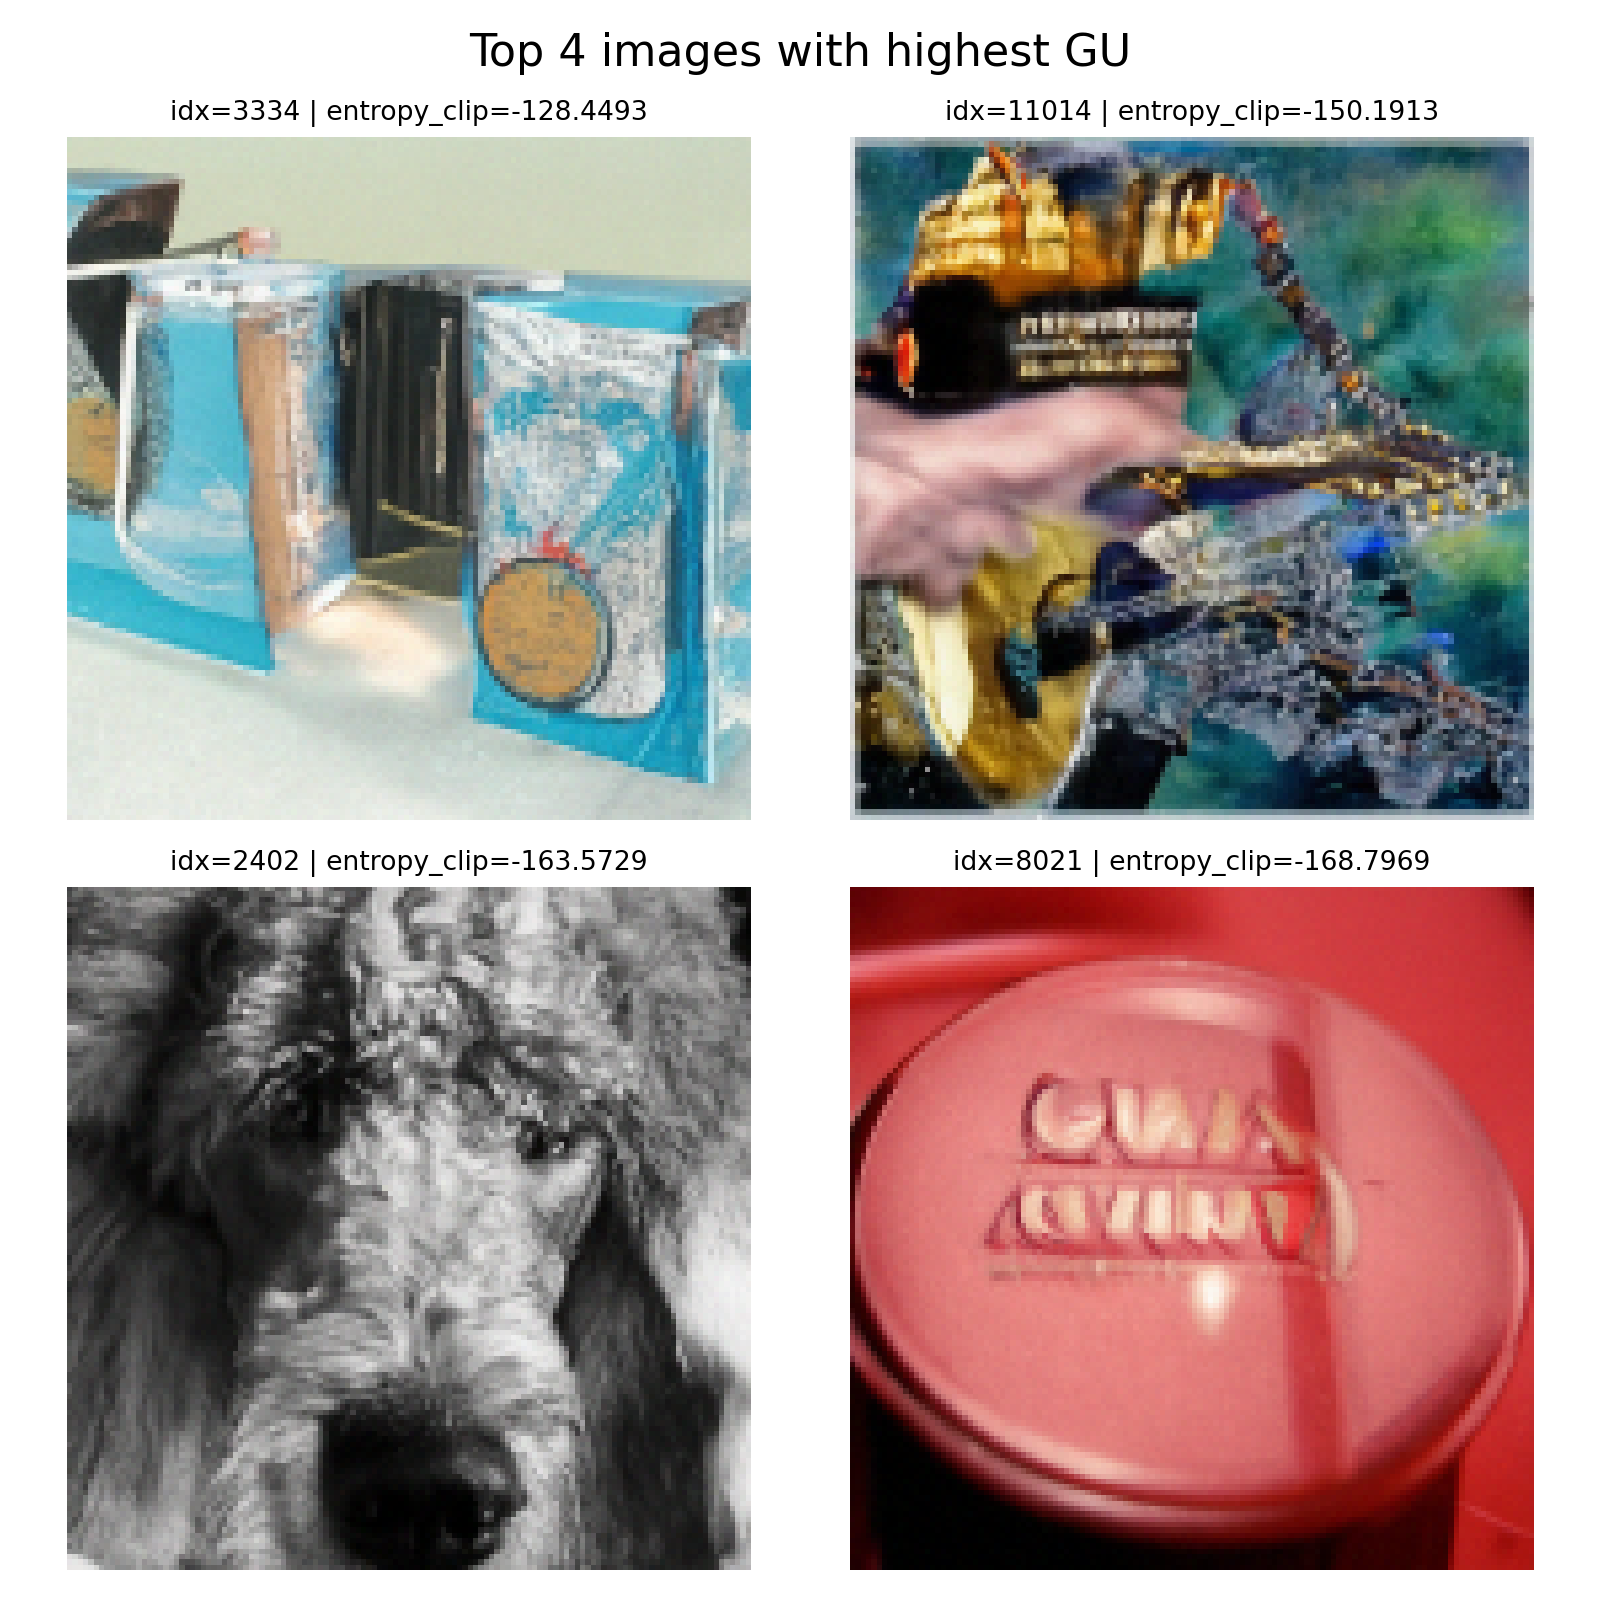
\includegraphics[width=\textwidth]{figures/introduction/worst_images_clip.png}
         \caption{Highest Uncertainty}
         \label{fig:intro_worst}
    \end{subfigure}
     % \hfill
    \begin{subfigure}[b]{0.47\textwidth}
         \centering
         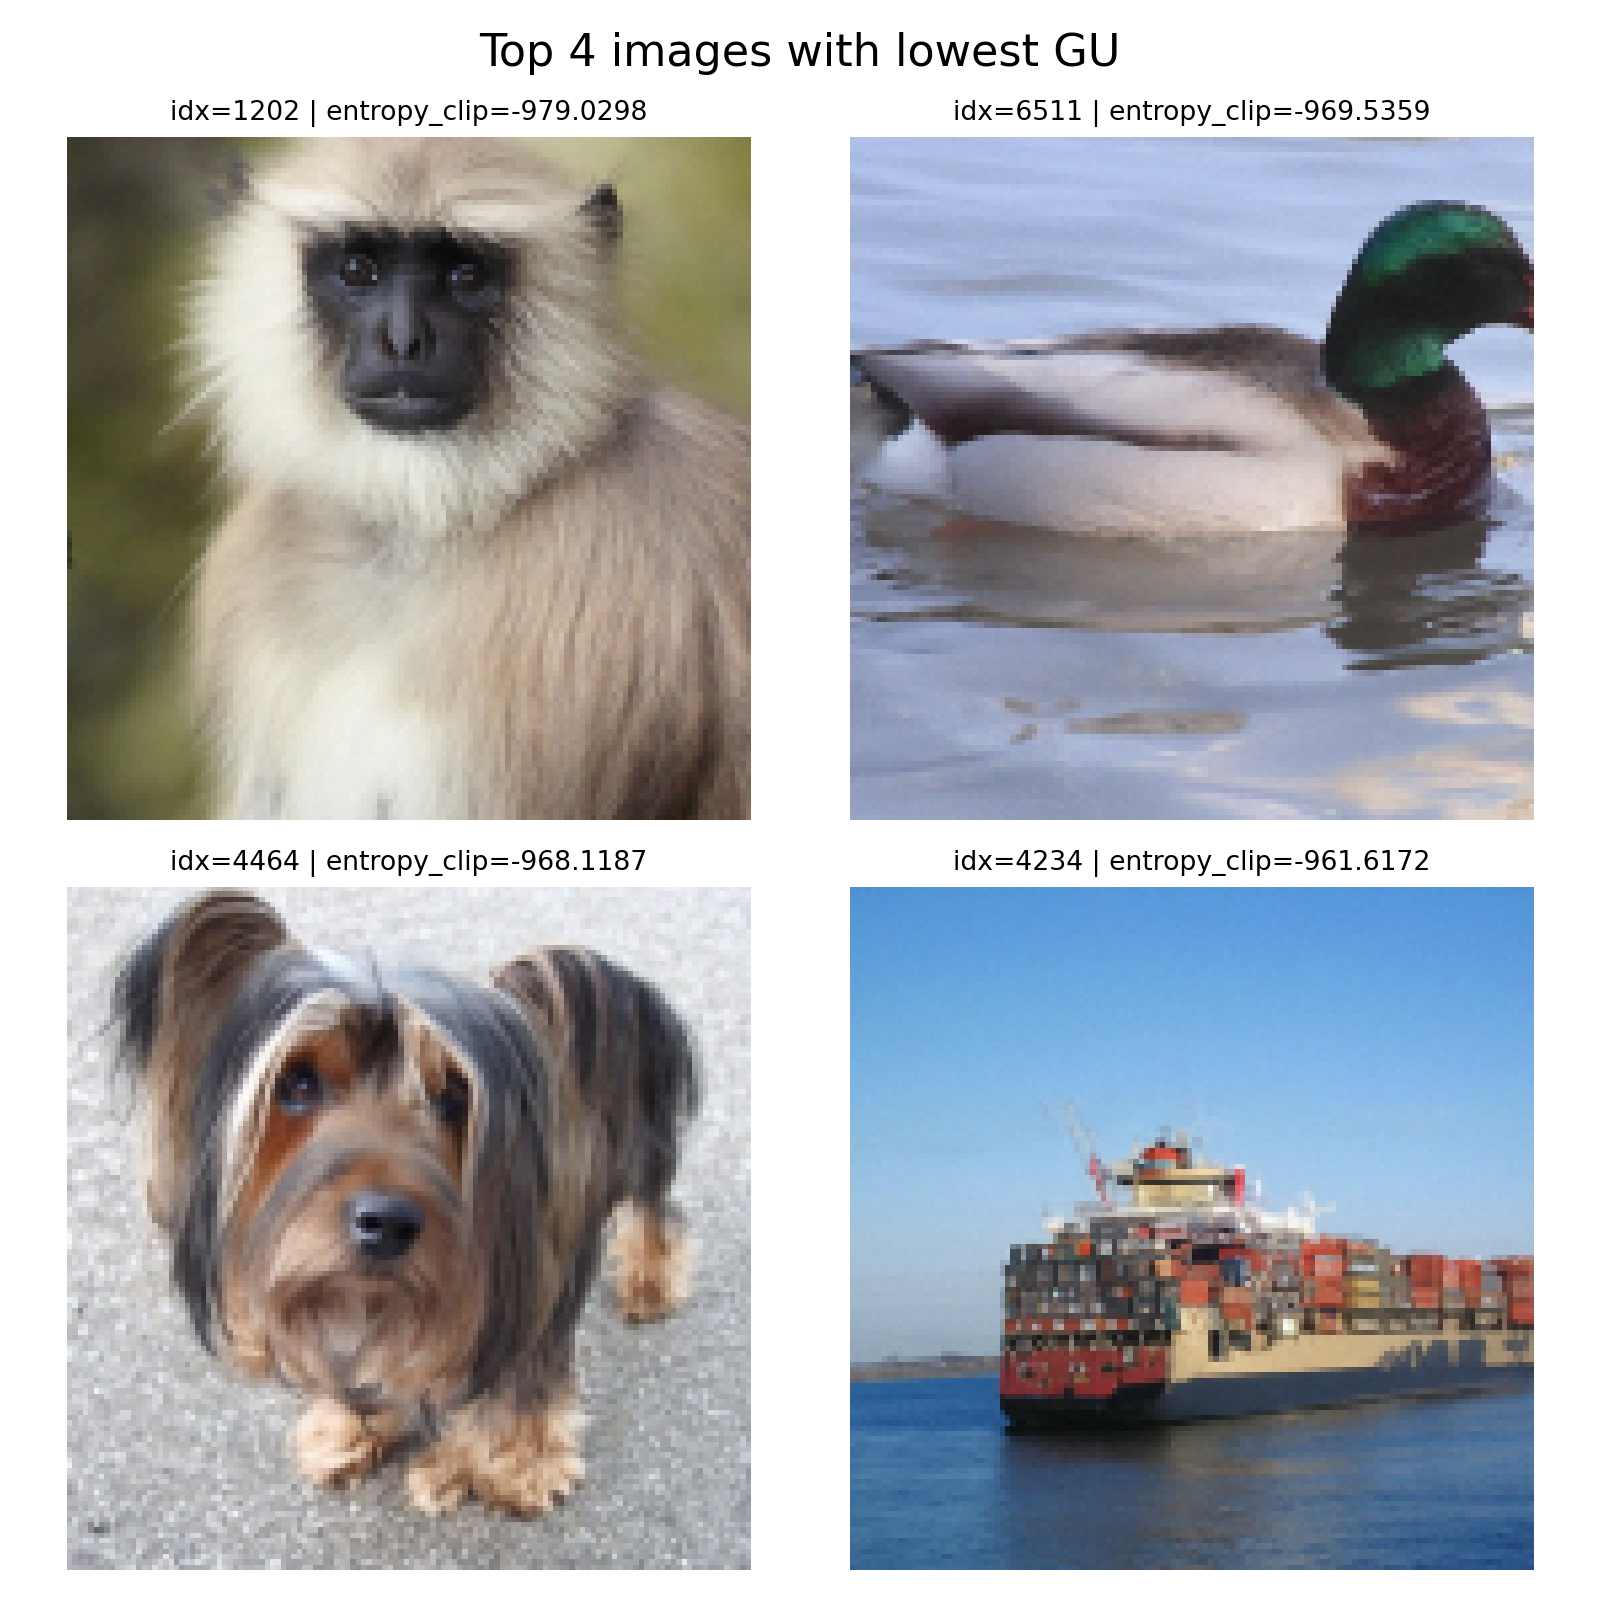
\includegraphics[width=\textwidth]{figures/introduction/top_images_clip.png}
         \caption{Lowest Uncertainty}
         \label{fig:intro_top}
    \end{subfigure}
    \caption{Taking the 4 most and least uncertain (w.r.t. \acs{GU}) images in a dataset 12032 generated images}
    \label{fig:intro_lowest_highest_gu}
\end{figure}

In this thesis, we use Bayesian machine (\autoref{sec:bg_bayesian}) learning to formulate \textit{Generative Uncertainty} (\acs{GU}): A measure of the model's output confidence that's tied to the confidence in the model's weights by formulating a posterior predictive distribution (prediction taking into account every possible weight configuration of the model) and evaluating it's variability. In the context of this thesis, \acs{GU} allows us to automatically identify and filter out weird\footnote{In this thesis, we define \textit{weird} with regards to human perception and assume that humans are good at deciding if an image belongs to the data distribution} looking or out-of-manifold\footnote{Images that are very different from what the model was trained on} natural images without the need for manual inspection, see \autoref{fig:intro_lowest_highest_gu}. And in the medical imaging \acs{GU} could be part of a safety mechanism, altering clinicians that a generated feature may be an artifact.

\paragraph{Objectives}

In this thesis we will investigate prior work and future work left by \cite{jazbec_generative_2025} that formulated a method to scale Bayesian machine learning methods to state of the art diffusion models. We will learn more about what \acs{GU} actually measure, what made \cite{jazbec_generative_2025} outperform previous methods, which assumptions made by \cite{jazbec_generative_2025} were wrong, their consequences and how to fix them.

% Bayesian machine learning (\autoref{sec:bg_bayesian}) appears as a capable framework to mitigate this risk with \textit{Generative Uncertainty}: A measure of the model's confidence in its own output that's tied to the confidence in it's model weights by formulating the posterior predictive distribution (that takes into account every possible weight configuration of the model) and evaluating it's variability. This system can isolate and flag highly uncertain samples. This can be part of a safety mechanism, alerting clinicians that a generated feature may be a model artifact rather than a true biological structure. 

% In the context of our work, adapting these Bayesian machine learning principles allows us to automatically identify and filter out weird\footnote{In this thesis, we define \textit{weird} with regards to human perception and assume that humans are good at deciding if an image belongs to the data distribution} looking or out-of-manifold\footnote{Images that are very different from what the model was trained on} natural images without the need for manual inspection \parencite{jazbec_generative_2025}.

% \section{Background}
% Generative models, such as Variational Autoencoders (VAEs) and Generative Adversarial Networks (GANs), aim to learn an underlying distribution of data to create new, synthetic samples. Diffusion models have recently emerged as a powerful class of generative models that produce high-quality data by reversing a progressive noise process (\autoref{sec:bg_diffusion}).

% State-of-the-art diffusion models can sometimes generate low-quality samples with severe artifacts. In critical applications like medical imaging, the model might hallucinate anatomical features or pathologies, potentially leading to severe diagnosis errors \parencite{xia_hallucinations_2025}. 

% Bayesian machine learning (\autoref{sec:bg_bayesian}) appears as a capable framework to mitigate this risk with \textit{Generative Uncertainty}: A measure of the model's confidence in its own output that's tied to the confidence in it's model weights by formulating the posterior predictive distribution (that takes into account every possible weight configuration of the model) and evaluating it's variability. This system can isolate and flag highly uncertain samples. This can be part of a safety mechanism, alerting clinicians that a generated feature may be a model artifact rather than a true biological structure. 

% In the context of our work, adapting these Bayesian machine learning principles allows us to automatically identify and filter out weird\footnote{In this thesis, we define \textit{weird} with regards to human perception and assume that humans are good at deciding if an image belongs to the data distribution} looking or out-of-manifold\footnote{Images that are very different from what the model was trained on} natural images without the need for manual inspection \parencite{jazbec_generative_2025}.

% \section{Prior work}

% \subsection{Uncertinaty Based}

% Recent research has actively debated how to implement and effectively scale Bayesian uncertainty estimation to large diffusion architectures.

% \begin{enumerate}
%     \item \textbf{Pixel-Space Epistemic Uncertainty}: BayesDiff \parencite{kou_bayesdiff_2024} started by applying a \textit{Last-Layer Laplace Approximation} (\acs{LLLA}) to track epistemic uncertainty throughout the diffusion sampling process. However, because BayesDiff computes uncertainty directly in the high-dimensional pixel space, it is overly sensitive to irrelevant background clutter rather than true semantic sample quality.
%     \item \textbf{Semantic Likelihood}: To resolve this dimensional challenge and background over-sensitivity, Jazbec et al. \parencite{jazbec_generative_2025} introduced a \textit{semantic likelihood}. By evaluating sample variability within the latent space of a pretrained feature extractor (e.g., CLIP), this framework successfully isolates semantic discordance and significantly outperforms pixel space methods in detecting low quality generations. \parencite{jazbec_generative_2025} Built upon BayesDiff but simplified their approach to only evaluate the uncertainty on the final timestep of the diffusion.
%     \item \textbf{Recent Critiques of \acs{LLLA}}: Despite these empirical successes, the reliance on \acs{LLLA} has recently faced pushback. \parencite{gupta_quantifying_2026} argue that \acs{LLLA} fails to sufficiently isolate epistemic from aleatoric uncertainty, proposing the FLARE (Fisher–Laplace
% Randomized Estimator) framework instead. Furthermore, \parencite{gegenfurtner_reducing_2026} demonstrate that simplistic approximations fail to capture the complex local geometry of the diffusion loss landscape leading to the sampling of bad (high loss) posterior samples (weigth sets), advocating instead for Riemannian approaches.
% \end{enumerate}

% Despite the criticism towards the \acs{LLLA}, \parencite{jazbec_generative_2025} will form the basis of this thesis. New ways of approximating the posterior distribution from \parencite{gegenfurtner_reducing_2026} and \parencite{gupta_quantifying_2026} are highly time consuming to implement and in the case of  \parencite{gupta_quantifying_2026} not proven to work on larger scale diffusion models such as ADM \parencite{dhariwal_diffusion_2021}. To fit within the relatively short time span of this master thesis, simpler ways of improving upon the LLLA will be explored.

% \parencite{jazbec_generative_2025} also suggested as future work to formalize the application of the Laplace Approximation and the semantic likelihood which has partially been done in \parencite{gegenfurtner_reducing_2026} through a Gibbs Posterior Framework.

% \subsection{Non-Uncertainty Based}

% Other, non-uncertainty based metrics to filter out bad samples exist. Those include realism \parencite{kynkaanniemi_improved_2019} and rarity \parencite{han_rarity_2022}. 

% In \parencite{jazbec_generative_2025} those metrics have been used as strong baselines to compare with Generative Uncertainty on multiple metrics (FID, Precision and Recall). Although they performed strongly on those metrics, sometimes outperforming Generative Uncertainty, they are exploiting the same exact embedding space as the aforementioned metrics, as opposed to Generative Uncertainty that uses a different embedding space, which would encourage using a new metric that would be independent of this embedding space to really test their usefulness.

\section{Prior work}

Prior work on scoring images samples quality mentioned throughout \cite{jazbec_generative_2025} can be sorted in two main categories: Bayesian based and Inception based.
The former is formed on the Bayesian machine learning the principle, the latter uses the latent space of the \texttt{Inception-v3} feature extractor to compares the generated samples distribution to the training/validation samples distribution.

\subsection{Bayesian Based}

Recent research has actively debated how to implement and effectively scale this Bayesian uncertainty estimation to large diffusion architectures.

\paragraph{Pixel-Space Epistemic Uncertainty} BayesDiff \parencite{kou_bayesdiff_2024} started by applying a \textit{Last-Layer Laplace Approximation} (\acs{LLLA}) (an approximation of the model's weights distribution) to track epistemic uncertainty (uncertainty stemming from the model's lack of knowledge) throughout the diffusion sampling process. The \acs{LLLA} makes this computationally feasible by treating only the final layer's weights as a probability distribution, rather than calculating this for the entire network. However, because BayesDiff computes uncertainty directly in the high-dimensional pixel space, it is overly sensitive to irrelevant background clutter rather than ``true'' semantic sample quality.

\paragraph{Semantic Likelihood} To resolve this dimensional challenge and background over-sensitivity, \cite{jazbec_generative_2025} introduced a \textit{semantic likelihood}. Rather than measuring uncertainty in pixel space, they evaluates whether the ``meaning'' of the generated image is stable. By evaluating sample variability within the latent space of a pretrained feature extractor (e.g., \acs{CLIP}), this framework successfully isolates semantic discordance instances where the model generates structural nonsense and significantly outperforms pixel space methods in detecting low-quality generations. \parencite{jazbec_generative_2025} built upon BayesDiff but simplified their approach to only evaluate the uncertainty on the final timestep of the reverse diffusion process.

\paragraph{Recent Critiques of LLLA} Despite these empirical successes, the reliance on \acs{LLLA} has recently faced pushback. \parencite{gupta_quantifying_2026} argue that \acs{LLLA} based uncertainty fails to sufficiently isolate epistemic uncertainty from aleatoric uncertainty (the inherent, irreducible randomness in the diffusion process itself), proposing the FLARE (Fisher–Laplace Randomized Estimator) framework instead. Furthermore, \parencite{gegenfurtner_reducing_2026} demonstrate that simplistic approximations such as \acs{LLLA} fail to capture the complex local geometry of the diffusion loss landscape, leading to an inaccurate distribution of model's weights that can give an high probability to a bad set of weights (one that's not actually associated to a low loss region). They advocate instead for a Riemannian approach that better map the true shape of the parameter space.

\paragraph{Where this thesis fits in}
Despite the criticism towards the \acs{LLLA}, \parencite{jazbec_generative_2025} will still form the basis of this thesis. New ways of approximating the posterior distribution from \parencite{gegenfurtner_reducing_2026} and \parencite{gupta_quantifying_2026} are highly time-consuming to implement and, in the case of \parencite{gupta_quantifying_2026}, not proven to work on larger scale, state of the art diffusion models such as the Ablated Diffusion Model (\acs{ADM}, \cite{dhariwal_diffusion_2021}). To fit within the relatively short time span of this master's thesis, simpler ways of improving upon the \acs{LLLA} will be explored.

% Outside of the considerations for the posterior approximation, this thesis will also address subjects left as future work \parencite{jazbec_generative_2025} such as:
% Formalizing the Bayesian model framework further and Using an internal feature extractor instead of relying on an external one which would allow the method to be used in many more fields where such external feature extractor is not available.
% \parencite{jazbec_generative_2025} also suggested as future work to formalize the application of the Laplace Approximation and the semantic likelihood, which has partially been done in \parencite{gegenfurtner_reducing_2026} through a Gibbs Posterior Framework.

\subsection{Inception Based}

Inception based metrics to filter out bad samples include realism \parencite{kynkaanniemi_improved_2019} and rarity \parencite{han_rarity_2022}. 
In \cite{jazbec_generative_2025}, those metrics have been used as strong baselines to compare with Generative Uncertainty (\acs{GU}) on the \acs{FPR} (FID, Precision, and Recall) set of metrics. Although they performed strongly on those metrics, sometimes outperforming Generative Uncertainty, they are exploiting the same exact embedding space as the aforementioned metrics. 
This is in contrast to Generative Uncertainty, which uses a different embedding space. This distinction among other issues described in \autoref{sub:problems_inception} encourage the use of a new metric that is independent of this embedding space.

\section{Thesis Plan}

This project focuses on formalizing and incrementally improving upon the generative uncertainty framework of \cite{jazbec_generative_2025}. 
It target both areas of future work left by \cite{jazbec_generative_2025} and issues discovered while experimenting for this thesis.
To achieve this, the thesis will go through the following steps:

\paragraph{Theoretical Validation} Examine the mathematical validity of applying the Laplace Approximation to a diffusion model's loss which is an area of future work from \cite{jazbec_generative_2025}.

\paragraph{Baseline Replication} Replicate some of the results from \parencite{jazbec_generative_2025}. The idea is to setup a solid foundation, proven to produce the same results as \parencite{jazbec_generative_2025}, on which to extend upon. 

\paragraph{Extending the Framework} Once we have that solid foundation, we conduct a set of experiments to understand the method further and potentially improve the results:
\begin{enumerate}
    % \item the instance of the ADM diffusion model used in \cite{jazbec_generative_2025} is missing a classifier that usually helps guiding model to higher quality generations \parencite{dhariwal_diffusion_2021}.
    % We will integrate this missing classifier to improve the image quality across the sampled dataset and observe how much improvement to the \acs{FPR} metrics can be obtained. 
    \item \textbf{Integrating Classifier Guidance}: The ADM diffusion model instance used in prior work lacks a classifier, which typically helps guide the model toward higher-quality generations \parencite{dhariwal_diffusion_2021}. In \autoref{ch:classifier} we will integrate this missing classifier to improve overall image quality and observe the resulting impact on standard evaluation metrics (\acs{FPR}).
    % \item \acs{VLM} (Vision Language Model) metric and filtering method. Implement the HPSv3 VLM metric (a model trained to emulate a human preference score (\acs{HPS})) to evaluate the diffusion model's performance on individual images which helps on a couple of fronts:
    % \begin{itemize}
    %     \item the FID metric is a good simple metric to start with in the field of natural images generation but it has been criticized in the literature \parencite{jayasumana_rethinking_2024} to contradict humans. Precision and Recall are built on the same feature extractor as the FID and are therefore also affected by this criticism leading to the need for an alternative for the \acs{FPR} set of metrics.
    %     \item the \acs{FPR} metrics can only be computed on batches of generated samples. Testing the metric on small batches is brittle and creating big batches of images is very expensive. 
        % \item Avoiding the task of manually reviewing the images and their score to make sure the uncertainty scoring method is properly.
    % \end{itemize}
    \item \textbf{Implementing a Vision Language Model (\acs{VLM}) Metric}: In \autoref{ch:hpsv3}, we will introduce the HPSv3 metric to evaluate the diffusion model's performance on individual images. This provides a human-aligned, per-image evaluation standard that addresses the structural flaws and high computational costs associated with batch-scale Inception-based metrics (such as FID, Precision, and Recall), which are analyzed in detail in \autoref{sub:problems_inception}.
    % \item Posterior Refinement. Implement targeted improvements to the \acs{LLLA} in a toy experiment (small diffusion model) context and measuring the effects of each of those changes with on metrics made for the toy experiment.
    % If a change seem to work really well on the toy instance, it may be tried on the much bigger ADM model and measured against the \acs{FPR} and \acs{HPS} metrics.
    \item \textbf{Refining the Posterior Approximation}: In \autoref{ch:toy_exp_posterior}, we will implement targeted improvements to the Last Layer Laplace Approximation (\acs{LLLA}) within a toy experiment. Modifications that demonstrate significant performance gains wil then be evaluated against the larger ADM model.
    % by for instance:
    % \begin{itemize}
    %     \item Adding more semantically rich layers to the posterior instead of only the last layer.
    %     \item Sampling weights randomly across the whole network instead of choosing a limited set of layers.
    %     \item Trying different approximation for the covariance matrix of the Laplace Approximation \acs{LA}
    % \end{itemize}
\end{enumerate}

% \paragraph{Experiments Motivated by Discoveries}

% While extending the framework, a question rose on the effect of one of the main contribution from \cite{jazbec_generative_2025}: as mentioned in prior work, they used a pretrained feature extractor to help the generative uncertainty metric be less sensitive to irrelevant background noise. We however realize in \autoref{ch:semantic-encoder} that this feature extractor made the whole Bayesian method$\star$ appear redundant, it was indeed possible to get very close to \cite{jazbec_generative_2025} results without measuring the uncertainty from the diffusion model but rather by only probing the feature extractor.

% \begin{tcolorbox}[colback=red!10!white,colframe=red!50!black,sharp corners]
% $\star$ The Bayesian method went through heavy approximations in \cite{jazbec_generative_2025} which might have made its uncertainty signal too weak to measure, especially after a pretrained feature encoder that alters the signal even more.
% This will be discussed further in later chapters (\ref{ch:toy_exp_posterior}, \ref{ch:semantic-encoder}, \ref{ch:using_internal_encoder}).
% \end{tcolorbox}

% This motivated an experiment to try and use a feature extractor that's part of the diffusion model itself to see if we could make the Bayesian work again and actually measure the diffusion model's uncertainty.

% As a bonus, using an internal encoder was also an area of future work from \cite{jazbec_generative_2025}.


\paragraph{Uncovering the External Semantic Encoder Vulnerability}
While extending the framework, we investigated the impact of the pretrained feature extractor used by \cite{jazbec_generative_2025} to reduce \acs{GU} sensitivity to irrelevant background noise in the images. We found that this external encoder inadvertently masks the diffusion model's true uncertainty. In fact, in \autoref{ch:semantic-encoder} we show that the filtering results from \cite{jazbec_generative_2025} can be closely replicated by probing the external feature extractor alone, rendering the upstream Bayesian methodology largely redundant.

We hypothesize that the heavy approximations applied to the Bayesian method explained in \autoref{sec:bg_gu_further_approx} weaken the uncertainty signal to the point that it is almost lost when passed through an external encoder. To correct this and accurately capture the diffusion model's inherent uncertainty, we propose utilizing an internal encoder native to the diffusion model. This experiment not only tests the viability of an uncontaminated uncertainty signal but also tackles an explicit area of future work proposed in the original study.

% the effect of using a pretrained feature extractor (as in \cite{jazbec_generative_2025}). The subsequent discovery made the whole Bayesian framework appear irrelevant and an experiment had to be conducted to try and use parts of the diffusion model itself as feature extractor to make the Bayesian framework relevant again. This experiment was also an area of future work from \cite{jazbec_generative_2025}.